\documentclass[12pt,border=6pt]{standalone}
\usepackage{fontspec}
\setmainfont{BeVietnamPro}[Path=D:/IOT_Tools/downloads/fonts/,Extension=.ttf,UprightFont=*-Regular,BoldFont=*-Bold]
\usepackage{amsmath}
\usepackage{unicode-math}\setmathfont{Cambria Math}
\usepackage{xcolor}
\usepackage{tikz}
\usetikzlibrary{positioning,arrows.meta,shapes.geometric,shapes.misc,calc,fit,backgrounds,decorations.pathreplacing,shadows,3d,perspective}
\usepackage{tikz-3dplot}
\usepackage{pgfplots}\pgfplotsset{compat=1.18}
\usepgfplotslibrary{groupplots,fillbetween}
\definecolor{cDo}{HTML}{BB2025}\definecolor{cDoD}{HTML}{8E1418}\definecolor{cDoT}{HTML}{FCEBEC}
\definecolor{cXanh}{HTML}{326CE5}\definecolor{cXanhT}{HTML}{EAF0FC}
\definecolor{cLuc}{HTML}{15803D}\definecolor{cLucT}{HTML}{E6F4EA}
\definecolor{cVang}{HTML}{B45309}\definecolor{cVangT}{HTML}{FDF2E1}
\definecolor{cNavy}{HTML}{1E293B}\definecolor{cMuc}{HTML}{1F2937}\definecolor{cXam}{HTML}{4B5563}
\definecolor{cXamT}{HTML}{F3F4F6}\definecolor{cVien}{HTML}{DDE1E6}\definecolor{cTim}{HTML}{6D28D9}\definecolor{cTimT}{HTML}{F1EBFD}
\pgfplotsset{slide/.style={tick label style={font=\small}, label style={font=\small}, scaled ticks=false,
  /pgf/number format/fixed, /pgf/number format/use comma, /pgf/number format/1000 sep={\,},
  legend style={font=\small,draw=none,fill=none}, axis line style={cXam}, major tick style={cXam},
  grid style={cVien}}}
\pgfkeys{/pgf/number format/assume math mode=true}
\begin{document}
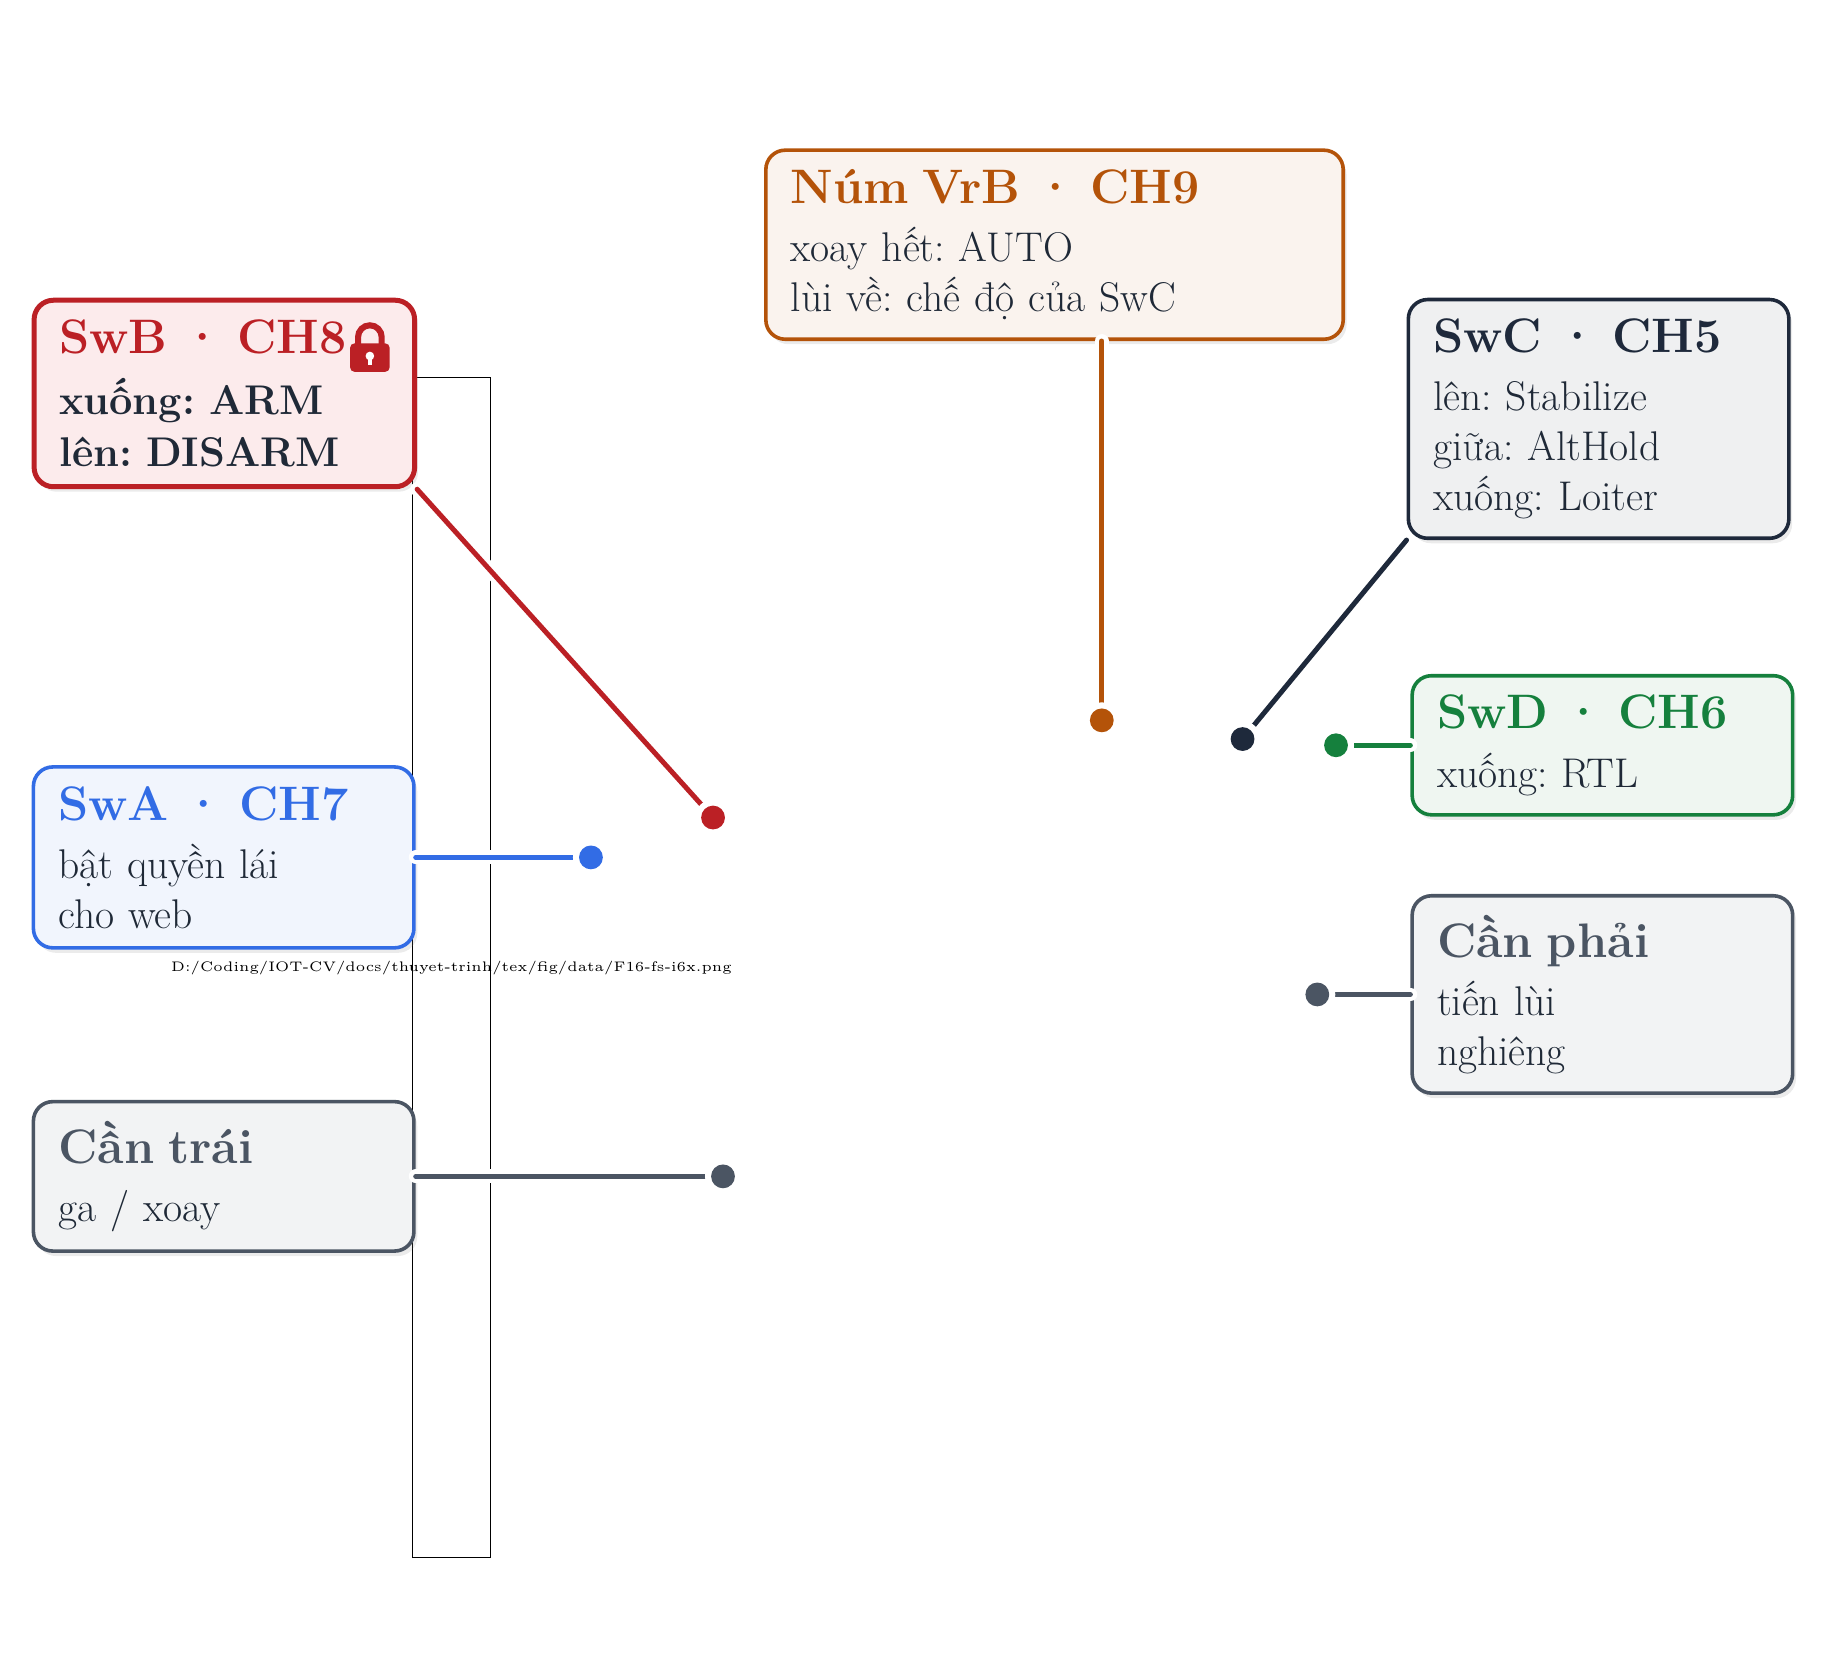
\begin{tikzpicture}[
  font=\fontsize{15}{18}\selectfont,
  card/.style={draw=#1, fill=#1!7, line width=1.3pt, rounded corners=7pt, inner xsep=9pt, inner ysep=7pt,
    text width=4.2cm, align=left, text=cMuc,
    drop shadow={opacity=0.16, shadow xshift=1.2pt, shadow yshift=-1.8pt}},
  halo/.style={white, line width=5pt, line cap=round},
  lead/.style={#1, line width=1.8pt, line cap=round},
]
\frenchspacing
% canvas 22,44 x 20,53 cm = the 9,0 x 8,25 in box of part_b (S14) minus the 6 pt border (scale 1 on the slide)
\def\W{22.44}\def\H{20.53}
\def\tit#1#2{{\color{#1}\bfseries\fontsize{17.5}{21}\selectfont #2}}
% ---------- photo (FS-i6X render cropped to 802 x 948 px, height 15 cm) ----------
\def\px{0.015823}
\node[anchor=north west, inner sep=0] at (4.875,16.1) {\pgfimage[height=15cm]{D:/Coding/IOT-CV/docs/thuyet-trinh/tex/fig/data/F16-fs-i6x.png}};
\begin{scope}[shift={(4.875,16.1)}, x=\px cm, y=-\px cm]
  \coordinate (pA) at (144,386);
  \coordinate (pB) at (242,354);
  \coordinate (pVrB) at (554,276);
  \coordinate (pC) at (667,291);
  \coordinate (pD) at (742,296);
  \coordinate (pL) at (250,642);
  \coordinate (pR) at (727,496);
\end{scope}
\coordinate (lx) at (0.05,0);
\coordinate (rx) at (\W-4.88,0);
% ---------- callout cards ----------
% left column
\node[card=cDo, fill=cDoT, line width=1.8pt, anchor=north west] (cB) at (0.05,17.1) {\tit{cDo}{SwB · CH8}\\[4pt]
  \textbf{xuống: ARM}\\[1pt] \textbf{lên: DISARM}};
\node[card=cXanh, anchor=west] (cA) at (lx |- pA) {\tit{cXanh}{SwA · CH7}\\[3pt]bật quyền lái\\cho web};
\node[card=cXam, anchor=west] (cL) at (lx |- pL) {\tit{cXam}{Cần trái}\\[3pt]ga / xoay};
% right column
\node[card=cNavy, anchor=north east] (cC) at (\W-0.05,17.1) {\tit{cNavy}{SwC · CH5}\\[3pt]
  lên: Stabilize\\ giữa: AltHold\\ xuống: Loiter};
\node[card=cLuc, anchor=west] (cD) at (rx |- pD) {\tit{cLuc}{SwD · CH6}\\[3pt]xuống: RTL};
\node[card=cXam, anchor=west] (cR) at (rx |- pR) {\tit{cXam}{Cần phải}\\[3pt]tiến lùi\\nghiêng};
% top centre
\node[card=cVang, anchor=south, text width=6.7cm] (cV) at ($(pVrB |- 0,16.55)+(-0.6,0)$) {\tit{cVang}{Núm VrB · CH9}\\[3pt]xoay hết: AUTO\\lùi về: chế độ của SwC};
% padlock on the SwB card
\begin{scope}[shift={($(cB.north east)+(-0.6,-0.62)$)}, cDo]
  \draw[line width=2.2pt] (-0.15,0.0) -- (-0.15,0.12) arc (180:0:0.15) -- (0.15,0.0);
  \fill[rounded corners=1.5pt] (-0.25,-0.32) rectangle (0.25,0.04);
  \fill[white] (0,-0.12) circle (0.055);
  \fill[white] (-0.025,-0.24) rectangle (0.025,-0.12);
\end{scope}
% ---------- leader lines ----------
\coordinate (vEnd) at (pVrB |- cV.south);
\foreach \p/\a/\c in {pB/cB.south east/cDo, pA/cA.east/cXanh, pL/cL.east/cXam, pC/cC.south west/cNavy,
                      pD/cD.west/cLuc, pR/cR.west/cXam, pVrB/vEnd/cVang}{
  \draw[halo] (\p) -- (\a);
  \draw[lead=\c] (\p) -- (\a);
  \fill[white] (\p) circle (6.5pt);
  \fill[\c] (\p) circle (4.3pt);
}
\pgfresetboundingbox
\useasboundingbox (0,0) rectangle (\W,\H);
\end{tikzpicture}

\end{document}
